\section{Řešení spolupráce s~YouTube API}
\subsection{YouTube Data API (v3)}
\par API v3\cite{apiv3} umožňuje začlenění informací YouTube do vlastní aplikace. Proto ho používám pro získání metadat. Nejprve jsem si~musel vytvořit google účet a~zaregistrovat aplikaci. Pro vytvoření google účtu a~zaregistrování slouží \url{https://console.developers.google.com/project}\cite{googleconsole}. Každý takto vytvořený projekt má u sebe statistiky s~počtem dotazů, počtem chyb, identifikačním řetězcem a~názvem. 
\par Po kliknutí na~název mého projektu je~možné se dozvědět podrobnější informace a~změnit konfiguraci projektu. Základní náhled mi poskytuje graf s~počtem požadavků, kde vidím, jak moc vytěžuji YouTube API\cite{apiv3}. Dále je~zde potřeba nechat si~vygenerovat unikátní API klíč, pomocí kterého získám přístup k~API a~tak mohu získávat metadata. Následující \hyperlink{consolesample}{obrázek 3.1} slouží jako ukázka pro úvodní stránku projektu.
\begin{figure}[h!]
	\hypertarget{consolesample}{}
	\centering
	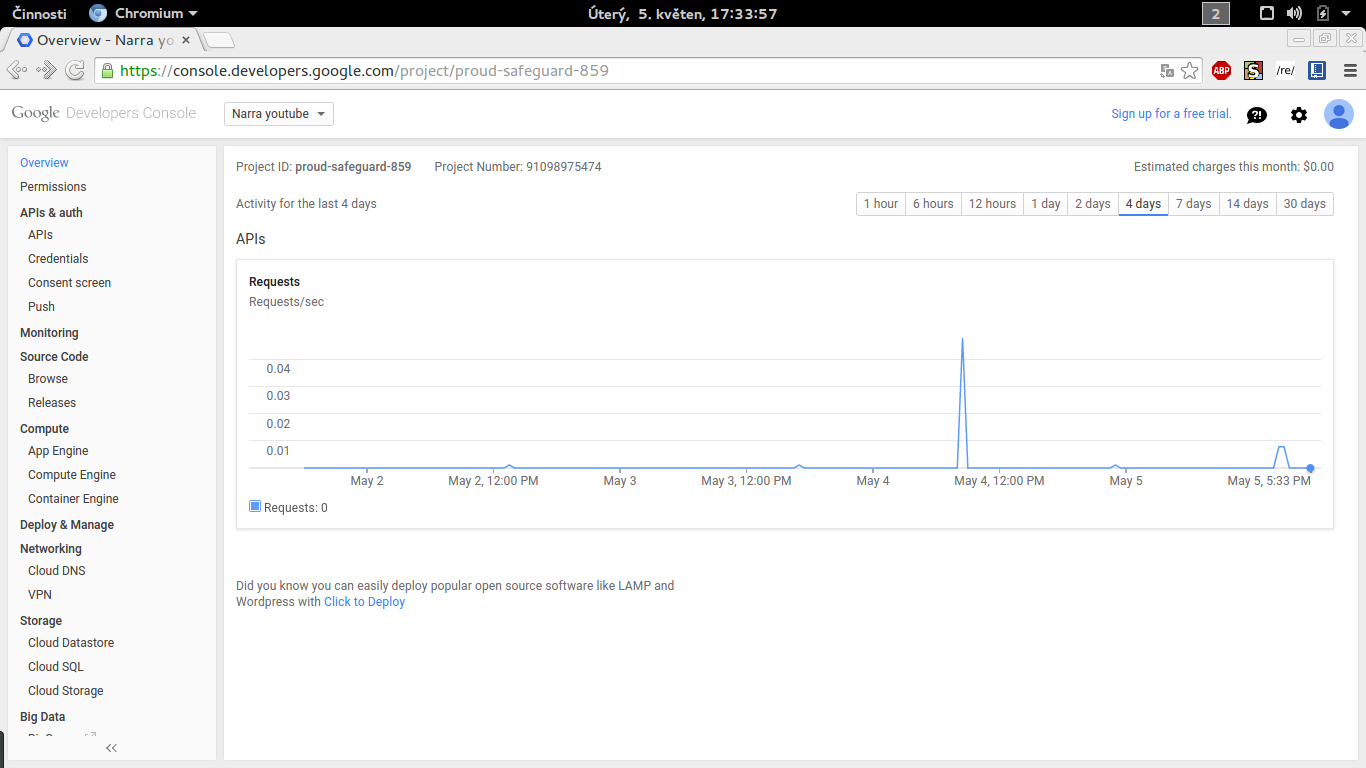
\includegraphics[width=\textwidth]{obrazova_priloha/my_projekt.png}
	\caption{Ukázka projektu na~google konzoli}
\end{figure}

\section{Třída connector}
\subsection{Založení aplikace}
\par Před založením aplikace jsem několikrát navštívil Michala Mocňáka, který se podílí na~vývoji projektu NARRA a~po vymyšlení mé části aplikace jsem požádal vedoucího práce, aby mi daný projekt předpřipravil, neboť na~\texttt{fork} projektu z NARRA jsem neměl dostatečná práva. Pro lehčí kontrolu mého postupu a~možnost verzování jsem zvolil službu GitHub \url{www.github.com}\cite{git}. Po předpřipravení projektu podle mého návrhu jsem si~na GitHubu vytvořil účet, přidal vlastní SSH klíč a~mohl jsem si~celou aplikaci k~sobě natáhnout a~začít programovat.

\subsection{Validace a~inicializace}
\par Vlastní implementace je~napsaná v~jazyce Ruby. Pro můj vývoj jsem si~vybral vývojové prostředí RubyMine. Pro vyřešení metadat jsem si~vytvořil jednu třídu, kterou jsem napojil na~\texttt{narra-core}. Dále jsem potřeboval knihovny \texttt{Net/HTTP} a~\texttt{JSON} pro snazší práci.
\begin{minted}{ruby}
require 'narra/core'
require 'net/http'
require 'json'

module Narra
  module Youtube
    class Connector < Narra::SPI::Connector
\end{minted}
\par Tímto kusem kódu jsem vytvořil nový modul, který je~potomkem Narra::\\SPI::Connector. Další věc jsem musel řešit validaci URL. V případě nevalidní URL mi stačilo vrátit false, při úspěchu jsem vracel true. Booleovskou hodnotu jsem použil, neboť musím umět říci konektoru zda umím či neumím danou URL obsloužit. Nejdřívě jsem zkoušel do metody validace URL zakomponovat metodu match. Ta ovšem vracela řetězec, který se shodoval, nebo hodnotu \texttt{nil} místo booleovké hodnoty a~proto jsem ji musel nahradit \verb|=~|. Takto zkonstruovaný výraz by ovšem nefungoval úplně dokonale, neboť při funkční URL by vrátil 0, což značí pozici od, které se výrazy shodují. Stačilo výraz lehce poupravit do tvaru !!(url \verb|=~| RegExp ) a~už jsem měl požadovaný booleovský výraz s~hodnotami true/false.
\begin{minted}{ruby}
!!(url =~ /^(?:http:\/\/|https:\/\/)?(www\.)?(youtu\.be\/|youtube
\.com\/(?:embed\/|v\/|watch\?v=|watch\?.+&v=))((\w|-){6,11})(\S*)
?$/
\end{minted}
\subsubsection{Regulární výraz pro validaci}
\par Regulární výraz\cite{regexp} je~matematický formalismus pro popis slov/vět jazyků. Jedná se tedy o~způsob, jak formálně popsat určité slovo, případně větu pomocí formálního vyjádření speciálními symboly a~skupinami znaků. V Ruby\cite{ruby} je~popis regulárním výrazem uvozen / na~začátku a~/ na~konci. Pomocí dvou lomítek řekneme překladači, že~zápis uvnitř lomítek má považovat za regulární výraz.
\par V předchozím regulárním výrazu jsem použil standardní konstrukce až~na jednu výjimku, která není tak častá. Jedná se o~?:(výraz), což znamená, že~bude splněno při žádném nebo jednom výskytu (výrazu). Tento způsob zápisu umožňuje kvantifikovat výskyt výrazu uvozené závorkami. Například \texttt{URL} \url{https://edux.fit.cvut.cz}, ve které mě nezajímá protokol, vytáhnu regulárním výrazem \texttt{(?:http/https)(edux.fit.cvut.cz)}. \hyperlink{regtable}{Tabulka 3.1} popisuje ostatní konstrukce regulárních výrazů v~jazyce Ruby. Pro otestování regulárních výrazů existuje velmi hezky zpracovaná stránka \url{http://rubular.com/}\cite{michaellovitt}.

\begin{center}
\begin{longtable}{| m{.20\textwidth} | m{.73\textwidth} |}
\hline
\verb|[abc]| & Právě jeden znak z množiny: a, b, c. \\
\hline
\verb|[^abc]| & Právě jeden znak z doplňku množiny: a, b, c. \\
\hline
\verb|[a-z]| & Právě jeden znak z rozsahu a-z. \\
\hline
\verb|[a-zA-Z]| & Právě jeden znak z rozsahu a-z nebo A-Z. \\
\hline
\verb|^| & Znak pro začátek řádky. \\
\hline
\verb|$| & Znak pro konec řádky, např \verb|[a-z]+$| bude uspokojen všemi řetězci tvořenými znaky a-z, který se vyskytne alespoň jednou a~bude před koncem řádky. \\
\hline
\verb|\A| & Začátek řetězce. \\
\hline
\verb|\z| & Konec řetězce. \\
\hline
\verb|.| & Jakýkoli znak. \\
\hline
\verb|\s| & Jakýkoli znak tvořený bílými znaky. \\
\hline
\verb|\S| & Jakýkoli znak netvořený bílými znaky. \\
\hline
\verb|\d| & Číslice. \\
\hline
\verb|\D| & Vše krom číslice. \\
\hline
\verb|\w| & Jakýkoli znak z množiny (písmeno, číslo, podtržítko). \\
\hline
\verb|\W| & Opak \verb|\w|. \\
\hline
\verb|\b| & Shoda musí nastat na~hranici číselného a~nečíselného znaku. \\
\hline
\verb|(...)| & Musí se shodovat přesně s~výrazem v~(), např (http)* značí nula až~nekonečno opakování http. \\
\hline
\verb|(a|b)| & Znak a~nebo b, a~i b mohou být i skupina znaků. \\
\hline
\verb|a?| & Žádný, nebo právě jeden výskyt a. \\
\hline
\verb|a*| & Žádný, nebo více výskytů znaku a. \\
\hline
\verb|a+| & Jeden, nebo více výskytů znaku a. \\
\hline
\verb|a{3}| & Přesně tři výskyty znaku a. \\
\hline
\verb|a{6,}| & Šest a~více výskytů znaku a. \\
\hline
\verb|a{3,6}| & Mezi třemi a~šesti výskyty znaků a. \\
\hline
\caption[Tabulka skupin symbolů pro regulární výraz]{Tabulka skupin symbolů pro regulární výraz}\label{tab:regexpr}
\end{longtable}
\end{center}

\par Pro správnou funkčnost ověření, zda je~URL validní či ne, bylo potřeba vyřešit přesměrování. Například URL adresa, která nevypadá ani z části jako validní, může vést k~videu na~serveru YouTube. Příkladem takové adresy je~\url{http://goo.gl/TKMZjS}. Pouhým ověřením přes regulární výraz bych neměl šanci zjistit obsah a~validitu odkazu. 

\subsection{Přesměrování}
\par Přesměrování\cite{nethttp} vyžadovalo novou knihovnu \texttt{NET/HTTP}, ze které jsem použil její zabudované metody. Při vytváření jsem nastavil horní hranici přesměrování na~20. Dále jsem potřeboval zajistit detekci smyček v~přesměrování, k~čemuž by docházet nemělo a~je to patologický příklad, ale je~dobré smyčku zdetekovat co nejdříve. Řešení pomocí pole je~pro takto málo prvků efektivnější, neboť HashMapa má větší nároky na~inicializaci v~porovnání s~jednoduchým polem. 
\par Číselné porovnání vypadá takto: vkládání do pole je~v~konstantním čase $\mathcal{O}(1)$, kdežto HashMapy je~v~nejhorším až~$\mathcal{O}(n)$. Na druhou stranu vyhledávání v~poli je~vždy $\mathcal{O}(n)$, kdežto HashMapy je~průměrně $\mathcal{O}(n * log(n))$ a~nejhůře také $\mathcal{O}(n)$. Protože u výpočtu složitosti jsou u HashMapy vysoké konstanty je~paměťově a~časově lepší zvolit pole. Takto se mohu podívat, zda jsem již nenavštívil nějakou URL dvakrát, což by znamenalo zacyklené přesměrování a~v mém případě vyhození příslušné vyjímky, neboť vím, že~takovouto URL nemohu nikdy zpracovat.

\par První úskalí knihovny \texttt{NET/HTTP}\cite{nethttp} nastalo v~okamžiku, kdy URL neměla v~názvu protokol. V tomto případě nebyla schopna rozpoznat server a~celý proces zkolaboval. Řešením bylo přidat k~URL bez protokolu protokol http, který se v~případě potřeby přesměruje na~https. Kdybych přidal místo pouhého http rovnou https, mohlo by se stát, že~některé stránky nebudou fungovat, neboť není zaručené zpětné přesměrování z šifrovaného protokolu na~nešifrovaný. Tohle bude platit hlavně u \uv{zkracovačů} URL (URL shorteners), které nepotřebují navazovat zabezpečené spojení. Pro vysvětlenou: HTTPS je~stále protokol HTTP, nad kterým je~spouštěna vrstva SSL šifrování.
\par Poslední část přesměrování spočívala ve zjištění příslušného kódu, kterým mi stránka odpověděla na~\texttt{GET} pořadavek. Při kódu 2xx je~vše v~pořádku a~URL lze rovnou vrátit. Stavový kód začínající trojkou je~ovšem zajímavějším, protože se jedná o~přesměrování. V tomto případě musí programátor zjistit, na~kterou stránku se dostane a~proces opakovat, než dostane kód 2xx, nebo než zjistí, že~je~v~cyklu, dostane chybový kód 4xx/5xx, či vyprší počítadlo přesměrování. Poslední skupina jsou kódy 4xx a~5xx značící chybu klienta nebo chybu serveru. Při chybách 4xx a~5xx vyhodím vyjímku, ve které uporozním na~výskyt kódu z tohoto rozsahu.

\subsection{Inicializace}
\par Po zjištění, zda je~požadovaná URL adresa validní, bylo potřeba ještě provést inicializaci. Při inicializaci se vytvoří instance objektu \texttt{Connector}, která zanikne až~v~momentě, kdy se všechna data přelijí do struktur databáze. Zde vytáhnu z YouTube API všechny potřebné informace o~videu, které budu dále zpracovávat. YouTube API nabízí parametrů, ze kterých si~můžu vybrat. Dále je~potřeba použít API klíč\cite{apistart}, pomocí něhož YouTube pozná, komu ubrat denní kvótu za požadavek. Toto řešení je~dočasné do doby, než v~jádře projektu NARRA doimplementují ověření pomocí \texttt{OAuth} a~každý uživatel bude mít kvůj vlastní vygenerovaný klíč. V následující tabulce\hyperlink{apiparams}{tabulce 3.2} je~příklad parametrů pro API.

\begin{table}[h!]
\hypertarget{apiparams}{}
\centering
\begin{tabular}{| l | l |}
\hline
\textbf{Parametr} & \textbf{Význam} \\
\hline
snippet & Zobrazí hlavní informace o~videu \\
\hline
contentDetails & Zobrazí detaily obsahu \\
\hline
fileDetails & Zobrazí detaily souboru \\
\hline
player & Zobrazí detaily přehrávače \\
\hline
processingDetails & Zobrazí podrobnosti zpracování \\
\hline
recordingDetails & Zobrazí podrobnosti nahrávání \\
\hline
statistics & Zobrazí statistiky videa \\
\hline
status & Zobrazí status \\
\hline
suggestions & Zobrazí návrhy \\
\hline
topicDetails & Zobrazí detaily o~tématu videa \\
\hline
\end{tabular}
\caption[Části dat YouTube API a~jejich význam]{Části dat YouTube API a~jejich význam}
\end{table}

\par Konrétní požavavek z mé aplikace na~YouTube API byl na~adresu \url{https://www.googleapis.com/youtube/v3/videos?id=#{@videoid}&key=můjklíč}\hfill \break \url{&part=část}\cite{apiurl}, kde \texttt{@videoid} je~inicializovaná hodnota pro identifikátor videa, můjklíč je~unikátní API klíč programátora, nebo v~budoucnosti uživatele systému NARRA a~část je~seznam požadovaných částí dat oddělených čárkou. Zde je~nutné vzít v~potaz, že~za vytížení YouTube serveru se platí a~v~jistých případech nemalou částí denní přidělené kvóty\cite{googleconsole1} jednotek. Detailní výpočet jsem popsal již v~kapitole o~YouTube API, zde se o~tomto omezení zmiňuji podruhé, neboť jsem nepoužil všech deset parametrů, ale jen čtyři. Cena použitých čtyř částí je~9 jednotek denní kvóty.
\par Část \texttt{snippet} vypíše o~videu většinu informací. \texttt{ContentDetails} byl potřeba pro splnění požadavků plynoucích z popisu v~DublinCore, \texttt{statistics} přidají do obsahu počty sledovaností a~\texttt{status} zobrazí licenci a~informace o~sdílení videa. Tyto čtyři položky stačí pro požadovaná metadata zadavatelem a~při přidání dalších bych zbytečně omezoval maximální počet vrácených položek díky omezení YouTube API a~aplikace by ztrácela na~efektivitě.
\par Při inicializaci je~druhý parametr klíč, který slouží k~autentizaci v~rámci YouTube API. Je nezbytný pro funkčnost, neboť při pořadavku na~informace o~videu musí mít YouTube možnost snížit konkrétnímu účtu denní kvótu.

\subsection{Parsování JSON objektu}
\par Nyní již mám k~dispozici JSON objekt a~můžu se pustit do práce. První pokus o~rozparsování proběhl ručně. Vždy jsem si~pomocí methody split rozdělil objekt na~pole o~dvou částech a~druhý index jsem rozdělil znovu podle čárky a~odřádkování. Pro lepší představu o~vizuální stránce kódu je~zde ukázka vytažení obsahu názvu videa:
\begin{minted}{ruby}
pom = @youtube_json_object_snippet.split('"title": "')[1]
@name = pom.split("\",\n")[0]
\end{minted}
\par Toto řešení bylo vcelku jednoduché, rozdělení podle ",\verb|\|n bylo v~pořádku, neboť YouTube v~popiscích provedlo escapacování těchto znaků a~nemohlo dojít k~nechtěnnému rozdělení ve špatném místě. Kód ovšem vypadal naprosto hrozně a~proto jsem zvolil již hotovou variantu JSON parseru. Pro porovnání ukázka kódu s~knihovnou JSON.
\begin{minted}{ruby}
my_hash = JSON.parse(@youtube)
my_hash["items"][0]["snippet"]["title"]
\end{minted}

\par Toto řešení je~mnohem přehlednější a~další programátor má usnadněné pochopení vnitřní struktury JSON objektu. Po této odbočce se dostáváme zpátky k~řešení, kde druhým zmiňovaným způsobem vracím název videa samostatně a~ne v~komplexní struktuře metadat. Tato alternativa byla zvolena záměrně díky ukládání videí v~mateřském projektu. Poskytnutí názvu videa v~podobě separátní metody je~nutností, protože Item (i potomci) musí mít název, kdežto metadata mít nemusí. Dalším požadavkem mateřského projektu bylo vrácení typu videa :video. Je to z toho důvodu, že~většina skriptů, které s~médiem dále pracují potřebují vědět, jestli je~to video, zvuk nebo obrázek. Tím jsem měl za sebou základní část a~mohl jsem pokračovat s~metadaty.

\subsection{Metadata}

\par Pro popis metadaty jsem vycházel ze struktury DublinCore, která ovšem ne úplně 100\% odpovídala mé představě ani představě YouTube vývojářů a~proto jsem celou kostru musel upravit. V tabulce 3.3 uvádím všechna metadata, která zpracovávám.

\begin{table}[!ht]
\centering
\begin{tabular}{| p{.28\textwidth} | p{.65\textwidth} |}
\hline
	\textbf{Název} & \textbf{Obsah} \\
\hline
\hline
	videoId & Jednoznačný identifikátor videa. \\
\hline
	channelId & Jednoznačný identifikátor kanálu, pod kterým je~video k~dispozici. \\
\hline
	channelTitle & Název kanálu, pod kterým je~video k~dispozici. \\
\hline
	publishedAt & Přesný čas vydání a~zvěřejnění videa. \\
\hline
	description & Popis k~videu. \\
\hline
	categoryId & Číslo kategorie, do které patří dané video. \\
\hline
	liveBroadcastContent & Booleovská hodnota, zda je~obsah ve videu vysílaný živě. \\
\hline
	viewCount & Počet shlédnutí videa. \\
\hline
	likeCount & Počet udělení líbí se. \\
\hline
	dislikeCount & Počet udělení nelíbí se. \\
\hline
	favouriteCount & Počet přidání do oblíbených. \\
\hline
	commentCount & Počet komentářů k~videu. \\
\hline
	duration & Čas trvání ve formátu \texttt{ISO\_8601}. \\
\hline
	dimension & Zda je~video 2d, nebo 3d. \\
\hline
	definition & Sd případně hd. \\
\hline
	caption & Booleovská hodnota, zda video obsahuje či neobsahuje titulky. \\
\hline
	licensedContent & Zda obsah videa podléhá licencování. \\
\hline
	regionRestriction & Zda je~video zakázané v~nějaká zemi. \\
\hline
	uploadStatus & Zda je~nahrané video již kompletní, či ještě ne. \\
\hline
	privacyStatus & Informace o~soukromí videa. \\
\hline
	license & Kdo vlastní licenci k~videu. \\
\hline
	embeddable & Zda je~možné toto video použít k~vložení. \\
\hline
	publicStatsViewable & Booleovská hodnota o~zobrazitelnosti veřejných statistik. \\
\hline
	timestamp & Čas ve formátu utc, kdy byla metadata pořízena. \\
\hline
\end{tabular}
\caption[Metadata předávaná do NARRA]{Metadata předávaná do NARRA}\label{tab:bson}
\end{table}

\par Jak jste si~mohli povšimnout v~této tabulce mi chybí titulek videa. Toto řešení je~součástí návrhu, kde vracím název videa samostatně pro lepší následné ukládání v~mateřském projektu. Dále mám staticky zadefinovaný typ videa, který se nemění. 
\par Pro správné pochopení, jak extrhahovat metadata ze struktury JSON objektu je~potřeba zjistit jak přesně vypadá. Celý objekt je~jeden prvek obsahující pole items, ze kterého používám nultý prvek. V této úrovni rozhoduji, zda vyberu data z položky snippet, statistics, contentDetails nebo status. Po zvolení například snippet se dostanu o~úroveň hlouběji a~mohu vybrat konkrétní položku, například channelId. Stejným způsoben jsou dostupná všechna metadata z JSON objektu, pouze u restrikce zemí vzacím složitější strukturu než string.
\par Poslední prvek metadat timestamp nenajdu v~DublinCore ani v~YouTube API, je~ovšem důležité ho do dat zařadit kvůli udržovatelnosti. V mateřské aplikaci bude nejspíš také časový otisk, který není v~této chvíli ještě dodělán a~proto jsem ho umístil do metadat. Je zde kvůli kontrole, jak staré jsou statistiky u videa a~například pro automatizovanou kontrolu metadat starších než dva týdny se tento údaj hodí. Ještě jsem přemýšlel, zda bude dobré řešení vložit časový otisk přímo do metadat nebo raději mimo, ale řešení s~otiskem v~metadatech vyhrálo. Nejpádnější důvod byl, že~při aktualizaci se zavolá pouze metoda metadata a~nebude se muset volat žádná další, neboť znovu stahovat video nemá cenu, v~případě přidání titulků se zavolá ještě download\_subtitles. Také jméno, identifikátor, URL a~typ videa se nebudou měnit.
\par Celkem můj gem poskytuje k~jednomu videu 24 metadat a~odděleně také jméno videa, typ videa. V součtu se jedná o~dvacet šest položek, které umožní rychlejší vyhledávání a~relevantní obsah pro každého uživatele, který moje rozšíření využije.

\par Pro správné pochopení, jak extrhahovat metadata ze struktury JSON objektu je~potřeba zjistit jak přesně vypadá. Celý objekt je~jeden prvek obsahující pole items, ze kterého používám nultý prvek, protože se ptám na~konkrétní video. V této úrovni rozhoduji, zda vyberu data z položky snippet, statistics, contentDetails nebo status. Po zvolení například snippet se dostanu o~úroveň hlouběji a~mohu vybrat konkrétní položku, například channelId. Stejným způsobem jsou dostupná všechna metadata z JSON objektu, pouze u restrikce zemí vracím složitější strukturu než řetězec (HashMapa s~prvky tvořenými polem).
\par Poslední prvek metadat timestamp nenajdu v~DublinCore ani v~YouTube API, je~ovšem důležité ho do dat zařadit, kvůli uživatelům. V mateřské aplikaci je~také časový otisk pro každé metadato, a~proto jsem ho umístil do metadat, kde jde o~uživatelky viditelnou informaci. Je zde kvůli kontrole, jak staré jsou statistiky u videa a~každý uživatel si~tak může ověřit, jak moc aktuální či neaktuální metadata jsou. V případě, že~by nastala chyba v~automatizované kontrole stáří metadat, je~také možné provést namátkovou oční kontrolu. Poslední metodou je~metoda pro stažení titulků download\_subtitles. Při aktualizování titulků předpokládám, že~pokud budou autoři YouTube opravdu používat jako úložiště, tak si~nebudou najednou měnit svůj systém značení médií.
\par Celkem můj gem poskytuje k~jednomu videu až~24 metadat a~odděleně také jméno videa, typ videa. V součtu se jedná o~dvacet šest položek, které umožní rychlejší vyhledávání v~systému NARRA a~poskytuje relevantní obsah pro každého uživatele, který moje rozšíření využije.

\subsection{Dokončení}
\par Na závěr mi zbývalo vrátit YouTube URL ve formátu, kde bude pouze video stream bez ostatních elementů, neboť ze standartní URL by to bylo moc práce navíc pro jádro aplikace. Pro tento účel souží adresa \url{#{env}/youtube_dl?id=#{@videoid}}. Proměnná env zde zastupuje proměnnou prostředí, která je~platná pro NARRA\_YOUTUBE\_SERVER a~videoid je~již dobře známý identifikátor videa.
\par Poslední kus kódu patřil stažení titulků. Na první pohled se to zdálo jako velmi jednoduchý úkol, ovšem stažení titulků stojí 200 jednotek. Proto je~potřeba autentizace API klíčem. Tímto klíčem je~potřeba být přihlášen již v~jádru aplikace při spuštění a~na můj konektor se jen dotázat na~stažení titulek. Jelikož je~ještě autentizace pomocí OAuth v~mateřském projektu nedořešená, předpřipravil jsem můj kus pro stažení titulek pouze pro aktuální funkčnost, která zabezpečí, že~po autentizaci pomocí OAuth začne mé stažení titulek fungovat.
\par Titulky k~videu jsou k~dispozici z \url{https://www.googleapis.com/youtube/v3/captions/}, za kterou se opět přiřadí identifikátor videa. Bez autorizace ovšem nahlásí stránka chybový kód: \uv{Login Required}.